% 文档类设置
\documentclass{ctexart}

% 导入宏包
\usepackage{hyperref} % PDF标签
\usepackage{graphicx} % 图片
\graphicspath{{images/}} % 图片路径
\usepackage{geometry} % 页面边距宏包
\geometry{left=3.17cm,right=3.17cm,top=2.54cm,bottom=2.54cm} % 页边距
\usepackage{fancyhdr} % 页眉页脚
\pagestyle{fancy} % 页面样式
\cfoot{\thepage} % 页脚中部
\renewcommand\headrulewidth{0pt}%隐藏页眉横线
\usepackage{enumerate} % 编号列表
\usepackage[simplified]{pgf-umlcd} % UML
\usepackage{listings} % 代码排版
\usepackage{dirtree} % 绘制树形目录
\usepackage{url} % 超链接
\usepackage{color,xcolor} % 颜色宏包
\usepackage[ruled]{algorithm2e} % 算法环境
% \usepackage{algorithmic} % 算法描述
% 代码块风格
\lstset{
    numbers=left,           % 行号
    numberstyle=\tiny,      % 行号样式
    basicstyle=\ttfamily,   % 基本代码风格
    breaklines=true,        % 自动换行
    keywordstyle=\bfseries\color{green!40!black}, % 关键字风格
    commentstyle=\itshape\color{gray}, % 注释的风格
    identifierstyle=\bfseries\color{blue}, % 标识符风格
    stringstyle=\color{orange}, % 字符串风格
    columns=fixed,
    frame=single, % 显示边框
    xleftmargin=\parindent,  % 左边距
    % xrightmargin=\parindent, % 右边距
    aboveskip=1em, % 顶部间隔
    captionpos=b % 文字提示符
}
\renewcommand{\lstlistingname}{代码}

% 算法描述的设置
\SetAlgorithmName{算法}{算法}{算法列表}
\SetKwInput{KwIn}{输入}
\SetKwInput{KwOut}{输出}
\LinesNumbered


% 角注设置
\renewcommand{\thefootnote}{\fnsymbol{footnote}}

% 章节标题设置
\ctexset{
    section = {
        format+ =  \zihao{-3} \raggedright,
        name = {,\quad},
        number = \arabic{section},
        aftername = \hspace{0pt}
    },
    subsection = {
        format+ =  \zihao{4} \raggedright,
        name = {,\quad},
        number = \arabic{section}.\arabic{subsection},
        aftername = \hspace{0pt}
    },
    subsubsection = {
        format+ =  \zihao{-4} \raggedright,
        name = {,\quad},
        number = \arabic{section}.\arabic{subsection}.\arabic{subsubsection},
        aftername = \hspace{0pt}
    }
}

% 封面页
\newcommand{\makecover}[4]{
    \begin{titlepage}
        \centering
        
\includegraphics[width=0.5\textwidth]{logo.png}\par
        \vspace{1cm}
        {\kaishu\ziju{0.1}\Huge 数学与计算机学院}\par
        \vspace{6cm}
        {\heiti\ziju{0.1}\zihao{0} #1}\par
        \vspace{6cm}
        {\kaishu\ziju{0.1}\Huge #2}\par
        \vspace{0.7cm}
        {\kaishu\Large #3}\par
        \vspace{1.5cm}
        {\kaishu\large #4}
    \end{titlepage}
}

% 画UML类图
% 参数2:文本宽度,参数3:类名,参数1:左上角坐标
\newenvironment{UMLClass}[3][0,0]
{
    \vspace{1em}\par\ttfamily
    \begin{tikzpicture}
        \begin{class}[text width=#2]{#3}{#1}
}
{
        \end{class}
    \end{tikzpicture}
    \vspace{1em}
}



\begin{document}
    % 产生封面
    \makecover{迷宫问题的求解报告}{杨鑫}{计算机11902班}{\today}

    \section{需求分析}

    \subsection{问题描述}

    以一个$m\times n$的长方阵表示迷宫,0和1分别表示迷宫中的通路和障碍。
    设计一个程序,对任意设定的迷宫,求出一条从入口到出口的通路,
    或得出没有通路的结论。

    \subsection{涉及知识点}
    求迷宫中从入口到出口的所有路径是一个经典的程序设计问题。由于计算机解迷宫时,
    通常用的是“穷举求解”的方法,即从入口出发,顺某一方向向前探索,若能走通,
    则继续往前走;否则沿原路径退回,换一个方向再继续探索,直至所有可能的通路都探索到为止。
    
    为了保证在任何位置上都能沿原路退回,显然需要用一个后进先出的结构来保存从入口到
    当前位置的路径。因此,在求迷宫通路的算法中应用“{\textbf 栈}”也就是自然而然的事了。
    
    \subsection{基本要求}
    \begin{enumerate}[\indent (1)]
        \item 首先实现一个以链表作存储结构的栈类型,然后编写一个求解迷宫的非递归程序。
        求得的通路以三元组$(i,j,d)$的形式输出。
        其中:$(i,j)$指示迷宫中的一个坐标,$d$表示走到下一坐标的方向。\par
        如,对于图 \ref{img:example} 所示的迷宫,输出一条通路为:
        $$(1,1,0),(1,2,1),(2,2,1),(3,2,2),(3,1,1),\cdots$$
        \item 编写递归形式的算法,求得迷宫中所有可能的通路。
        \item 以方阵形式输出迷宫及其通路。
    \end{enumerate}
    \begin{figure}[b]
        \centering
        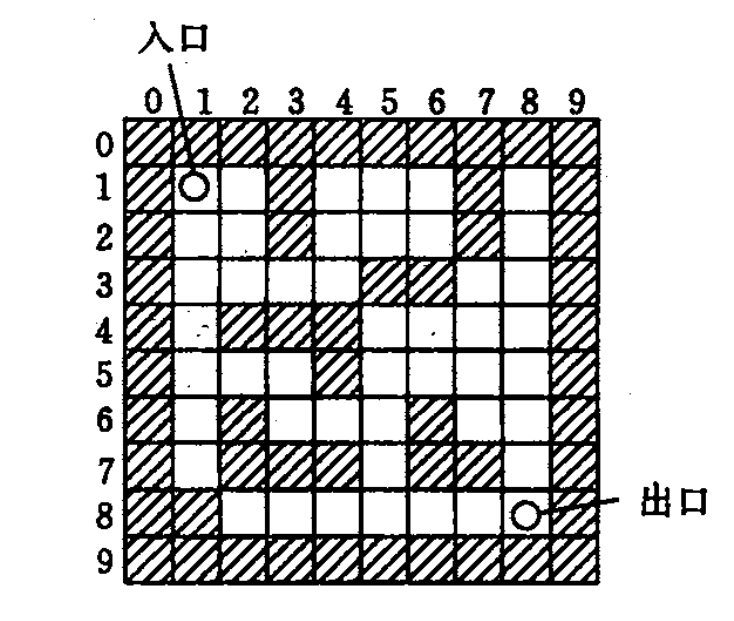
\includegraphics[scale=0.5]{迷宫示例.png}
        \caption{迷宫示例}
        \label{img:example}
    \end{figure}
    \section{概要设计}
    \subsection{数据结构}
    
    \subsubsection{坐标位置类}
    坐标是一个重要的数据结构,它记录了方块的位置信息,是计算机探索路径的关键依据。

    \begin{center}
        \begin{UMLClass}{8cm}{Pos}
            \attribute{+ i : int}
            \attribute{+ j : int}
            \operation{+ Pos()}
            \operation{+ Pos(int i, int j)}
            \operation{+ operator==(const Pos\& right) : bool}
            \operation{+ to\_String(): string}
        \end{UMLClass}
    \end{center}

    坐标类数据成员:(i,j)表示一个坐标,i和j均为int类型。
    
    坐标类函数成员:
    \begin{itemize}
        \item Pos(),构造函数,初始化一个坐标
        \item Pos(),有参构造函数,指定初始化一个坐标
        \item operator==(),重载“==”运算符,用于判断两个位置是否相等
        \item to\_String(),将坐标信息转换为字符串
    \end{itemize}

    \subsubsection{通道块类}

    假设“当前位置”指的是“在搜索过程中某一时刻所在图中某个方块位置”,那么
    应该有一个辅助变量指示计算机下一次要达到的位置。“下一位置”可以是当前
    位置的东、南、西、北方向相邻的方块,我们只记录即将转向的方向值就可以了。

    于是,将坐标位置和“从此通道块走向下一通道块的方向”封装成一个通道块类。

    规定,di的值为0、1、2、3,分别代表东、南、西、北。

    \begin{center}
        \begin{UMLClass}{10cm}{Block}
            \attribute{+ ord : int}
            \attribute{+ seat : Pos}
            \attribute{+ di : int}
            \operation{+ Block()}
            \operation{+ Block(int ord, Pos seat)}
            \operation{+ setBlock(int ord, Pos seat, int di)}
            \operation{+ to\_String() : string}
            \operation{+ operator<<(ostream\& out, Block block) : ostream\&}
        \end{UMLClass}
    \end{center}

    通道块类数据成员:
    \begin{itemize}
        \item ord,通道块在路径上的“序号”
        \item seat,通道块在迷宫中的“坐标”
        \item 从此通道块走向下一通道块的方向
    \end{itemize}

    通道块类函数成员:
    \begin{itemize}
        \item Block(),构造函数,初始化一个通道块
        \item setBlock(),设置通道块
        \item to\_String(),将通道块信息转换为字符串
        \item operator<<(),重载“<<”运算符,用于输出通道块类信息到输出流中
    \end{itemize}

    \subsubsection{迷宫类}

    将迷宫的行数、列数、迷宫矩阵,封装成一个迷宫类。
    此处规定迷宫矩阵中障碍的值为“@”,通路的值为“.”,计算机探索后,经过的路径的值为“*”。

    \begin{center}
        \begin{UMLClass}{8cm}{Maze}
            \attribute{- r : int}
            \attribute{- c : int}
            \attribute{- map : char[][]}
            \operation{+ Maze()}
            \operation{+ Maze(int r, int c, char map[][])}
            \operation{+ getRow() : int}
            \operation{+ getCol() : int}
            \operation{+ setRow()}
            \operation{+ setCol()}
            \operation{+ setMapValue(Pos pos, char value)}
            \operation{+ getMapValue(Pos pos) : char}
            \operation{+ canPass(Pos pos) : bool}
        \end{UMLClass}
    \end{center}

    迷宫类数据成员:
    \begin{itemize}
        \item r,行数
        \item c,列数
        \item map,迷宫矩阵
    \end{itemize}

    迷宫类函数成员:
    \begin{itemize}
        \item Maze(),构造函数,初始化迷宫
        \item getRow(),获取行数
        \item getCol(),获取列数
        \item setRow(),设置行数
        \item setCol(),设置列数
        \item setMapValue(),设置迷宫矩阵某坐标元素值
        \item getMapValue(),获取迷宫矩阵某坐标元素值
        \item canPass(),某坐标是否通路
    \end{itemize}

    \subsubsection{栈节点类}

    栈节点类,组成栈结构的基本单元,此处选用链栈结构。

    \begin{center}
        \begin{UMLClass}{8cm}{Node}
            \attribute{- data: T}
            \attribute{- next: Node<T>*}
            \operation{+ Node()}
            \operation{+ Node(T data, Node<T>* next = nullptr)}
            \operation{+ getData() : T}
            \operation{+ setNext(Node<T>* next)}
            \operation{+ getNext() : Node<T>*}
        \end{UMLClass}
    \end{center}

    栈节点类的数据成员:
    \begin{itemize}
        \item block,数据域
        \item next,指针域,指向下一节点
    \end{itemize}

    栈节点类的函数成员:
    \begin{itemize}
        \item Node(),构造函数,初始化一个节点
        \item getData(),获取数据域
        \item setNext(),设置下一节点
        \item getNext(),获取下一节点
    \end{itemize}

    \subsubsection{栈类}

    \emph{栈}(Stack),是限定仅在表尾进行插入或删除的线性数据结构,
    具有“后进先出”的特点。这符合迷宫问题求解时需在任何位置上都能沿原路退回的要求。

    这里使用栈的链式结构。

    \begin{center}
        \begin{UMLClass}{8cm}{Stack}
            \attribute{- top: Node<T>*}
            \attribute{- size: int}
            \operation{+ Stack()}
            \operation{$\sim $ Stack()}
            \operation{+ getSize() : int}
            \operation{+ isEmpty() : bool}
            \operation{+ push(T data)}
            \operation{+ pop()}
            \operation{+ pop(T \&e)}
            \operation{+ getTop() : Node<T>\&}
            \operation{+ print()}
        \end{UMLClass}
    \end{center}

    栈类的数据成员:
    \begin{itemize}
        \item top,栈顶,链栈头指针
        \item size,栈大小(节点个数)
    \end{itemize}

    栈类的函数成员:
    \begin{itemize}
        \item Stack(),构造函数,初始化一个栈
        \item $\sim $Stack(),析构函数,释放栈
        \item getSize(),获取栈长
        \item isEmpty(),判断栈是否为空
        \item push(),入栈
        \item pop(),出栈
        \item getTop(),获取栈顶
        \item print(),将栈输出到cout对象中
    \end{itemize}
    
    
    \subsection{程序模块}
    \begin{enumerate}
        \item 输入模块
         \par 从标准输入或文件中输入迷宫矩阵。
        \item 非递归搜索算法模块
         \par 使用栈这种数据结构进行路径的非递归搜索,
              求出一条路径或判定是否存在通路。
         \par 该算法的设计见算法\ref{alg1}。
         \begin{algorithm}[h]
            \caption{非递归搜索}
            \label{alg1}
            \KwIn{入口位置 start, 出口位置 end}
            \KwOut{迷宫矩阵的一条通路路径,或不存在通路}
            \SetKwRepeat{Do}{do}{while}
            Stack S\;
            当前位置 $curpos \gets start$\; 
            \Do{S不空}{
                \eIf{curpos 可通}{
                    $curpos$ 入栈\quad (纳入路径)\;
                    \eIf{curpos = end}{
                        STOP\;
                    }{
                        $curpos \gets$ 东邻居方块\;
                    }
                }{
                    \If{S 不空}{
                        \If{栈顶位置尚有其他方向未经探索}{
                            $curpos \gets$ 沿顺时针方向旋转找到的栈顶位置的下一相邻方块\;
                        }
                        \If{栈顶位置四周均不可通}{
                            S 栈顶出栈\quad (从路径中删去该通道块)\;
                            \If{S 不空}{
                                重新测试新的栈顶位置,
                                直至找到一个可通的相邻块或出栈至空栈; 
                            }
                        }
                    }
                }
            }
        \end{algorithm}
        \item 递归搜索算法模块
         \par 使用栈这种数据结构进行路径的递归搜索,
              求出所有通路路径。
         \par 该算法的设计见算法\ref{alg2}。
         \begin{algorithm}[htp]
            \caption{递归搜索}
            \label{alg2}
            \KwIn{入口位置 start, 出口位置 end}
            \KwOut{迷宫矩阵的一条通路路径,或不存在通路}
            \SetKwRepeat{Do}{do}{while}
            Stack S\;
            \SetKwFunction{path}{MazePath}
            \SetKwProg{Fn}{Function}{ is}{end}
            \Fn{\path{Pos start, Pos end}}{
                \eIf{start = end}{
                    $end$ 入栈\;
                    Print 当前通路路径\;
                    $end$ 出栈\;
                }{
                    \If{start 可通}{
                        \While{start 相邻方块未全部探索}{
                            $start$ 入栈\;
                            Pos $next \gets $ 沿顺时针方向的下一相邻方块\;
                            \path{next, end}\;
                            $start$ 出栈\;
                        }
                    }
                }
            }
        \end{algorithm}
    \end{enumerate}

    \section{详细设计}

    \subsection{类的函数实现}
    
    \subsubsection{坐标位置类}

    坐标位置类的函数实现如代码 \ref{code1} 所示。
\begin{lstlisting}[language=C++,caption=Pos类的实现,label=code1]
// 重载 "==" 运算符,用于判断两个位置是否相等
bool Pos::operator==(const Pos &right) const {
    return (i == right.i && j == right.j);
}
// 构造函数
Pos::Pos() : Pos(0, 0) {}
Pos::Pos(int i, int j) {
    this->i = i;
    this->j = j;
}
// 将坐标信息转换为字符串
std::string Pos::to_String() {
    return ( std::to_string(i) + "," + std::to_string(j));
}
\end{lstlisting}


    \subsubsection{通道块类}
    通道块类的函数实现如代码 \ref{code2} 所示。
\begin{lstlisting}[language=C++,caption=Block类的实现,label=code2]
// 构造函数
Block::Block() = default;
Block::Block(int ord, Pos seat, int di) {
    setBlock(ord, seat, di);
}
// 设置通道块
void Block::setBlock(int ord, Pos seat, int di){
    this->ord = ord;
    this->seat = seat;
    this->di = di;
}
// 将通道块信息转换为字符串
std::string Block::to_String() {
    return "("  + seat.to_String() + "," + std::to_string(di) + ")";
}
// 重载"<<"运算符,用于输出通道块类信息到输出流中
std::ostream &operator<<(std::ostream &output, Block block) {
    output << block.to_String();
    return output;
} 
\end{lstlisting}

    \subsubsection{迷宫类}
    迷宫类的函数实现如代码 \ref{code3} 所示。
\begin{lstlisting}[language=C++,caption=Maze类的实现,label=code3]
// 构造函数
Maze::Maze() = default;
Maze::Maze(int r, int c, char map[MAXLEN][MAXLEN]) {
    this->r = r;
    this->c = c;
    // 将map拷贝到this->map
    for (int i = 0; i < r; i++) {
        for (int j = 0; j < c; j++) {
            this->map[i][j] = map[i][j];
        }
    }
}
// 获取行数
int Maze::getRow() {
    return r;
}
// 获取列数
int Maze::getCol() {
    return c;
}
// 设置列数
void Maze::setRow(int row){
    this->r = row;
}
// 设置行数
void Maze::setCol(int col){
    this->c = col;
}
// 设置迷宫矩阵某坐标元素值
void Maze::setMapValue(Pos pos, char value) {
    this->map[pos.i][pos.j] = value;
}
// 获取迷宫矩阵某坐标元素值
char Maze::getMapValue(Pos pos) {
    return map[pos.i][pos.j];
}
// 某坐标是否通路
bool Maze::canPass(Pos pos) {
    return getMapValue(pos) == '.';
}
\end{lstlisting}

    \subsubsection{栈节点类}
    栈节点类的函数实现如代码 \ref{code4} 所示。
\begin{lstlisting}[language=C++,caption=Node类的实现,label=code4]
// 构造函数
template<typename T>
Node<T>::Node() = default;
// 有参构造函数
template<typename T>
Node<T>::Node(T data, Node<T> *next) {
    this->data = data;
    this->next = next;
}
// 获取数据域
template<typename T>
T Node<T>::getData() {
    return data;
}
// 设置下一节点
template<typename T>
void Node<T>::setNext(Node<T> *next) {
    this->next = next;
}
// 获取下一节点
template<typename T>
Node<T> *Node<T>::getNext() {
    return next;
}
\end{lstlisting}

    \subsubsection{栈类}
    栈类的函数实现如代码 \ref{code5} 所示。
\begin{lstlisting}[language=C++,caption=Stack类的实现,label=code5]
// 构造函数
template<typename T>
Stack<T>::Stack() {
    top = nullptr;
    // 初始时,没有节点
    size = 0;
}
// 析构函数
template<typename T>
Stack<T>::~Stack() {
    while (top) { // 如果栈顶存在
        Node<T> *p = top;
        top = top->getNext();
        // 释放栈顶
        delete p;
    }
}
// 判断栈是否为空
template<typename T>
bool Stack<T>::isEmpty() {
    return top == nullptr;
}
// 获取栈长
template<typename T>
int Stack<T>::getSize(){
    return size;
}
// 入栈
template<typename T>
void Stack<T>::push(T data) {
    // 生成新栈顶,并指向当前栈顶
    auto newTop = new Node<T>{data, top};
    // top指向新栈顶
    top = newTop;
    // 更新size
    size++;
}
// 出栈
template<typename T>
void Stack<T>::pop() {
    if (isEmpty()) {
        std::cerr << "栈空! 无法出栈." << std::endl;
        exit(1);
    }
    Node<T> *p = top;
    // top变为原栈顶的下一节点
    top = top->getNext();
    // 删除原栈顶
    delete p;
    // 更新size
    size--;
}
// 出栈并将栈顶节点的data值赋给参数e
template<typename T>
void Stack<T>::pop(T &e) {
    if (isEmpty()) {
        std::cerr << "栈空! 无法出栈." << std::endl;
        exit(1);
    }
    // 将栈顶赋值给e
    e = (*top).getData();
    Node<T> *p = top;
    // top变为原栈顶的下一节点
    top = top->getNext();
    // 删除原栈顶
    delete p;
    // 更新size
    size--;
}
// 获取栈顶的引用
template<typename T>
Node<T> &Stack<T>::getTop() {
    if (isEmpty()) {
        std::cerr << "栈空! 没有栈顶." << std::endl;
        exit(1);
    }
    return *top;
}
// 打印栈
template<typename T>
void Stack<T>::print() {
    if (isEmpty()) {
        std::cout << "null";
    }
    Node<T> *p = top;
    auto cnt{1};
    while (p) {
        std::string ch = (cnt % 5 ? " " : "\n"); // 一行五个
        if (cnt == size) // 如果是最后一个
            ch = "\n";
        cnt++;
        std::cout << p->getData() << ch;
        p = p->getNext();
    }
}
\end{lstlisting}

    \subsection{程序模块}

    \subsubsection{输入模块}
    输入模块的函数代码实现如代码 \ref{code6} 所示。
\begin{lstlisting}[language=C++,caption=输入模块,label=code6]
/**
* @brief 输入迷宫
* @param maze 迷宫对象,将输入到此对象中
* @param In 流对象,从此流对象输入到maze中
*/
void InputMaze(Maze &maze, std::istream &In) {
    auto row{0}, col{0};
    In >> row >> col;
    maze.setRow(row);
    maze.setCol(col);
    char value;
    for (int i = 0; i < maze.getRow(); i++) {
        for (int j = 0; j < maze.getRow(); j++) {
            In >> value;
            maze.setMapValue(Pos{i, j}, value);
        }
    }
}
\end{lstlisting}


    \subsubsection{非递归搜索算法模块}
    根据算法 \ref{alg1} 的设计,编写出了相应的C++语言代码,见代码 \ref{code7}。
\begin{lstlisting}[language=C++,caption=非递归搜索算法模块代码,label=code7]
Status MazePath(Maze &maze, Pos start, Pos end) {
    Stack<Block> S;     // 实例化一个栈对象
    Pos curpos = start; // 当前坐标
    Block e;            // 实例化一个通道块对象
    int curstep = 1;    // 探索步骤

    do {
        if (maze.canPass(curpos)) {         // 当前位置可通过
            maze.setMapValue(curpos, '*');  // 留下足迹
            e.setBlock(curstep, curpos, 0); // 设置待入栈的通道块

            S.push(e); // 入栈
            if (curpos == end) { // 到达终点(出口)
                S.print();
                return true;
            }
            // 下一位置是当前位置的东邻
            curpos = NextPos(curpos, 0);
            // 探索下一步
            curstep++;
        } else { // 当前不能通过
            if (!S.isEmpty()) {
                S.pop(e); // 出栈
                while (e.di == 3 && !S.isEmpty()) {
                    if (maze.getMapValue(e.seat) != '@')
                        maze.setMapValue(e.seat, '.');
                    S.pop(e); // 出栈,回退一步
                }
                if (e.di < 3) {
                    e.di++; // 换下一个方向探索
                    S.push(e);
                    // 设定当前位置是该新方向上的相邻块
                    curpos = NextPos(e.seat, e.di);
                }
            }
        }
    } while (!S.isEmpty());
    return false;
}
\end{lstlisting}

    \subsubsection{递归搜索算法模块}
    根据算法 \ref{alg2} 的设计,编写出了相应的C++语言代码,见代码 \ref{code8}。
\begin{lstlisting}[language=C++,caption=递归搜索算法模块代码,label=code8]
Maze maze;
Stack<Block> S;
int count = 0; // 路径计数

void ReMazepath(Pos start, Pos end) {
    if (start == end) {
        // 放入终点
        maze.setMapValue(start, '*');
        S.push(Block{S.getSize() + 1, start, 1});
        cout << "找到第" << ++count << "条通路:" << endl;
        S.print();
        PrintMaze(maze);
        // 退出栈,找下一条路径
        S.pop();
        // 恢复原值
        maze.setMapValue(start, '.');
    } else {
        if (maze.canPass(start)) {
            int di = 0;
            while (di < 4) {
                // 加入当前方块
                S.push(Block{1, start, di});
                // 下一位置
                Pos next = NextPos(start, di);
                // 避免来回走动
                maze.setMapValue(start, '*');
                // 递归
                ReMazepath(next, end);
                // 退出栈,找其他元素
                S.pop();
                // 恢复原值
                maze.setMapValue(start, '.');
                di++;
            }
        }
    }
}
\end{lstlisting}

    \subsection{其他函数}
    \emph{NextPos} 函数,用于确定下一相邻方块:
\begin{lstlisting}[language=C++,caption=NextPos函数,label=code9]
int dir[][2] = {{0,  1},   // 东
                {1,  0},   // 南
                {0,  -1},  // 西
                {-1, 0}};  // 北

Pos NextPos(Pos curpos, int i) {
    Pos ret = curpos;
    // 新坐标
    ret.i += dir[i][0];
    ret.j += dir[i][1];
    return ret;
}
\end{lstlisting}

    \emph{PrintMaze} 函数,打印迷宫路程图:
\begin{lstlisting}[language=C++,caption=PrintMaze函数,label=code10]
void PrintMaze(Maze &maze) {
    std::cout << "迷宫路程图: \n";
    for (int i = 0; i < maze.getRow(); i++) {
        std::cout << "      ";
        for (int j = 0; j < maze.getCol(); j++) {
            std::cout << std::setw(2)
                      << maze.getMapValue(Pos{i, j});
        }
        std::cout << std::endl;
    }
    std::cout << std::endl;
}
\end{lstlisting}

    \emph{main} 函数、\emph{menu} 函数、重载的 \emph{InputMaze} 函数,
    用于组织程序结构:
\begin{lstlisting}[language=C++,caption=其他函数,label=code11]
int main() {
    while (true) {
        switch (menu()) {
            case 1: {
                InputMaze();
                Pos start, end;
                cout << "输入入口位置:";
                cin >> start.i >> start.j;
                cout << "输入出口位置:";
                cin >> end.i >> end.j;
                auto flag = MazePath(maze, start, end);
                if (flag) {
                    PrintMaze(maze);
                } else {
                    cout << "*****    此迷宫无法从起点走到终点。   ******\n";
                }
            }
                break;
            case 2: {
                InputMaze();
                Pos start, end;
                cout << "输入入口位置:";
                cin >> start.i >> start.j;
                cout << "输入出口位置:";
                cin >> end.i >> end.j;
                ReMazepath(start, end);
            }
                break;
            case 0:
                cout << "程序结束,谢谢使用!" << endl;
                exit(0);
        }
    }
    return 0;
}

int menu() {
    auto sn{0};
    cout << endl
            << "<---------------显示菜单---------------" << endl
            << "1. 非递归搜索迷宫通路路径" << endl
            << "2. 递归搜搜迷宫通路路径" << endl
            << "0. 结束程序" << endl
            << "---------------显示菜单--------------->" << endl
            << "输入0-2:";
    while (true) {
        cin >> sn;
        if (sn < 0 || sn > 3)
            cout << "输入错误,重选0-2:" << endl;
        else
            break;
    }
    return sn;
}

void InputMaze() {
    auto way{0};
    cout << "0手动输入,1从文件导入:";
    while (true) {
        cin >> way;
        if (way < 0 || way > 1)
            cout << "输入错误,重新输入0或1:" << endl;
        else
            break;
    }
    if (way) {
        std::string filename;
        cout << "输入文件名:";
        cin >> filename;
        std::ifstream InputFile;
        InputFile.open(filename);
        if (!InputFile.is_open()) {
            std::cerr << "没有找到文件" << filename << endl;
            exit(1);
        }
        InputMaze(maze, InputFile);
        InputFile.close();
    } else {
        cout << "输入行数、列数、迷宫矩阵:" << endl;
        InputMaze(maze, std::cin);
    }
}
\end{lstlisting}
    
    \section{测试分析}

    使用 G++ 8.1.0 编译器编译本实例,运行测试。

    测试文件为 test.in ,其内容见图 \ref{img:maze} :

    \begin{figure}[h]
        \centering
        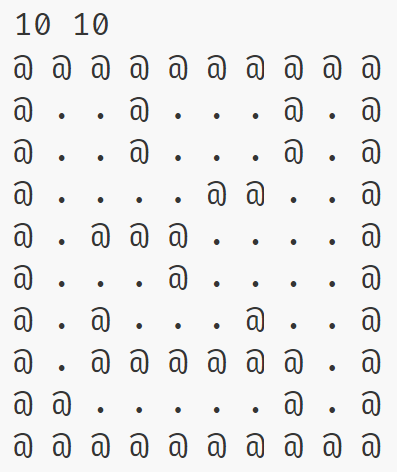
\includegraphics{迷宫.png}
        \caption{测试迷宫}
        \label{img:maze}
    \end{figure}

    \subsection{非递归搜索}
    \subsubsection{搜索成功}
    
    入口:(1,1),出口(8,8),结果见图\ref{img:test1}。

    \begin{figure}[h]
        \centering
        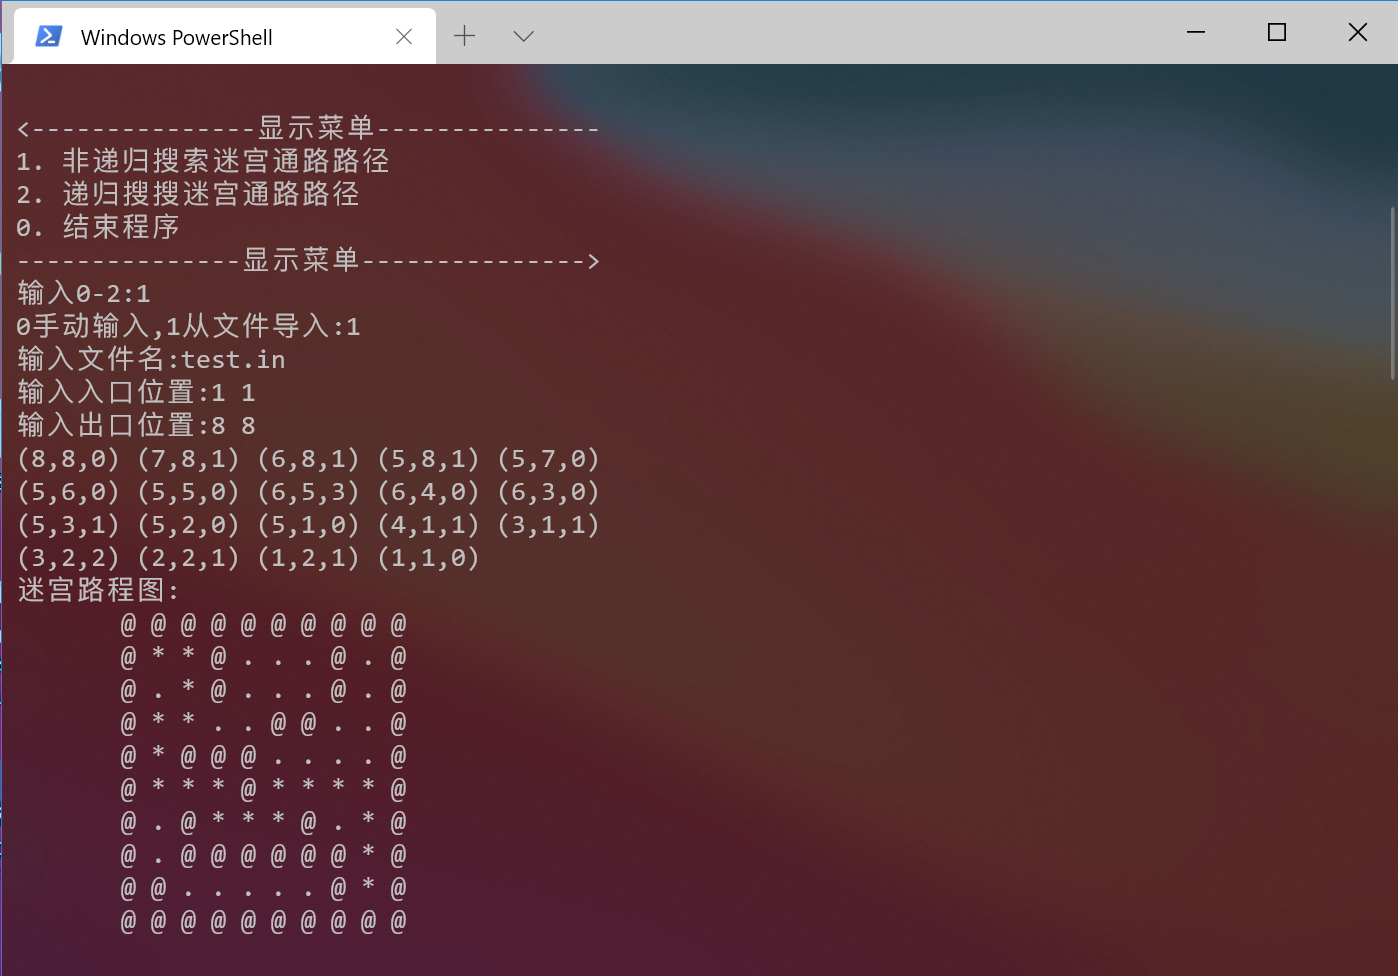
\includegraphics[width=0.7\textwidth]{测试结果1.png}
        \caption{非递归搜索 - 搜索成功}
        \label{img:test1}
    \end{figure}

    \subsubsection{搜索失败}

    入口:(1,1),出口(9,3),结果见图\ref{img:test2}。

    \begin{figure}[h]
        \centering
        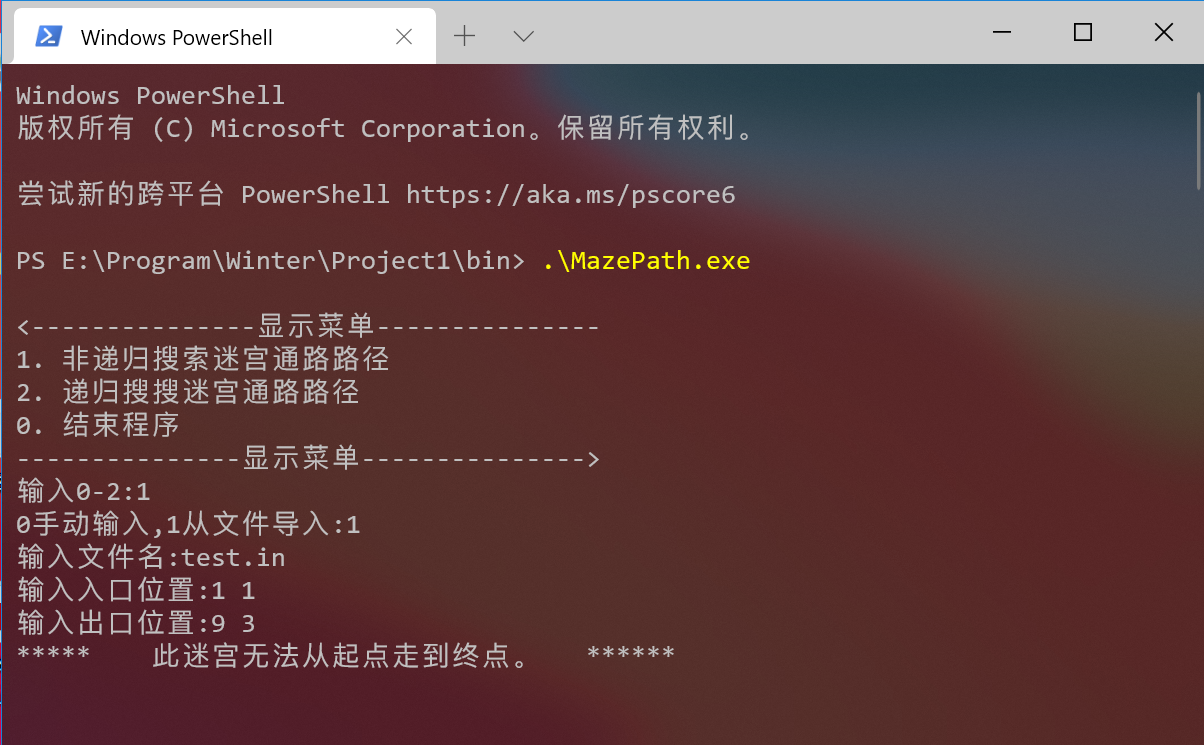
\includegraphics[width=0.7\textwidth]{测试结果6.png}
        \caption{非递归搜索 - 搜索失败}
        \label{img:test2}
    \end{figure}


    \section{递归搜索}

    入口:(1,1),出口(6,4),共有4条通路路径,结果见图 \ref{img:test3} 和图 \ref{img:test4}。

    \begin{figure}[h]
        \centering
        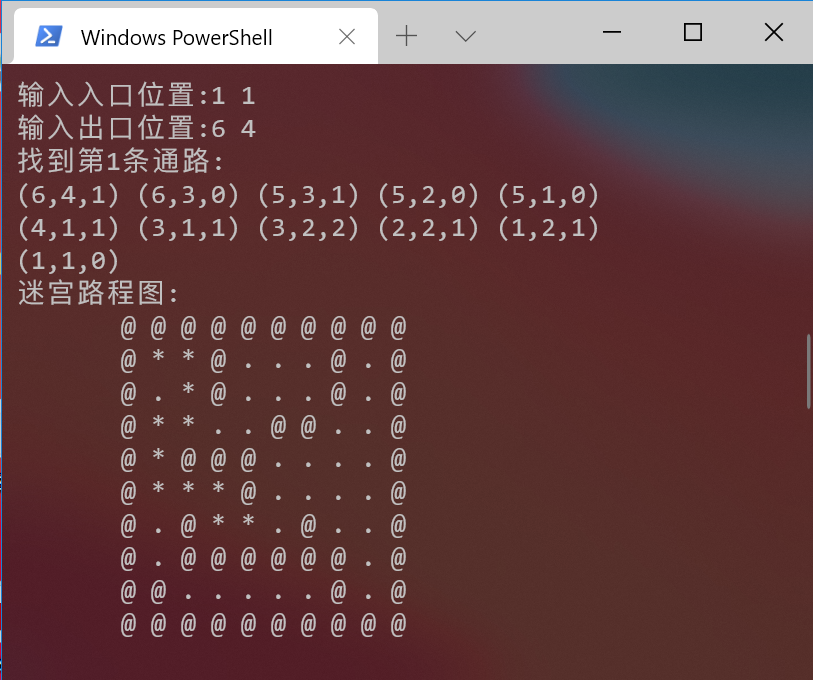
\includegraphics[width=0.47\textwidth]{测试结果2.png}
        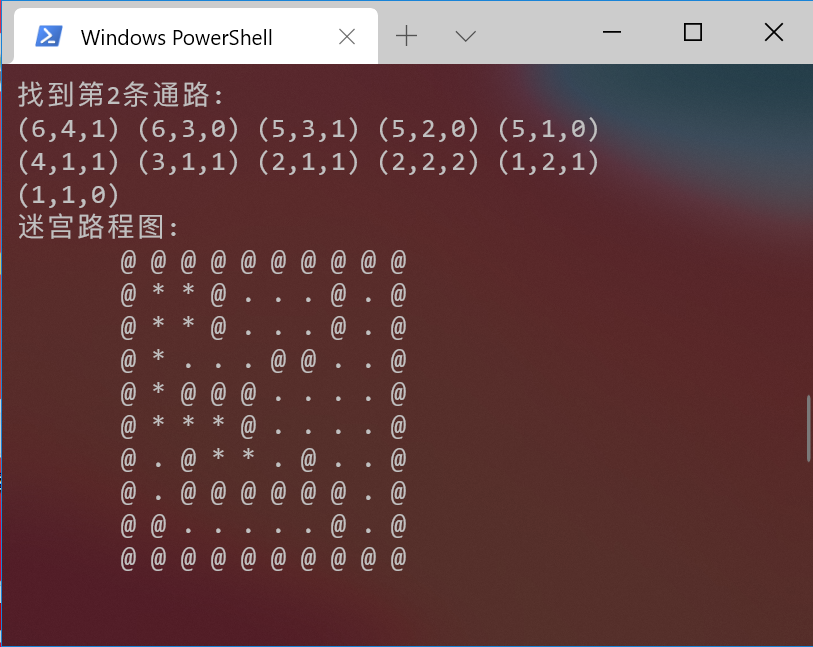
\includegraphics[width=0.5\textwidth]{测试结果3.png}
        \caption{递归搜索 - 第一条和第二条通路路径}
        \label{img:test3}
    \end{figure}
    \begin{figure}[h]
        \centering
        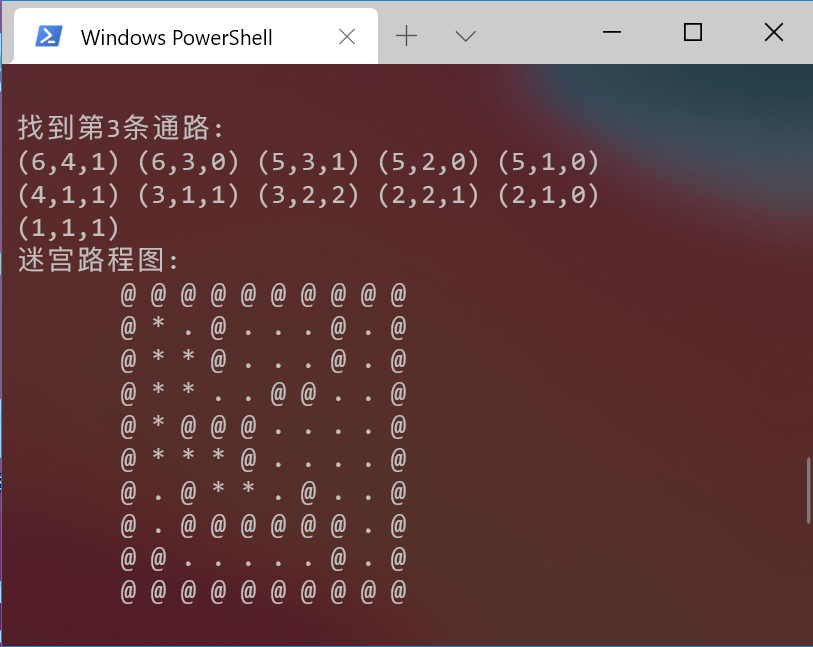
\includegraphics[width=0.47\textwidth]{测试结果4.png}
        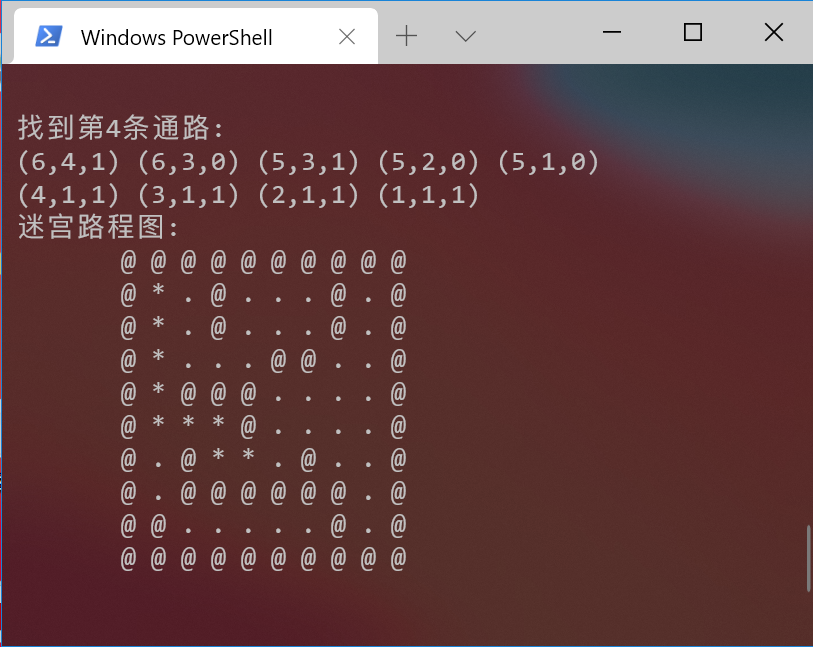
\includegraphics[width=0.47\textwidth]{测试结果5.png}
        \caption{递归搜索 - 第三条和第四条通路路径}
        \label{img:test4}
    \end{figure}

    \section{总结}

    通过本次项目实践,熟练地掌握栈了这种数据结构,并实现了链栈的编写。
    
    使用计算机进行迷宫通路路径的探索,使得栈这种数据结构得到实际的应用。
    在实践过程中,使用了非递归搜索算法,对计算机如何模拟实际问题有了较好的
    感性理解。在使用递归搜索算法中,感受到了递归所带来了的便利之处,能够将
    复杂的问题简单化,并且也易于人理解。

    \section{附录}

    本项目实例使用CMake构建,并要求编译器为 G++ 8.1.0,使用的操作系统是 Windows。
    
    项目主要文件清单:
    
    \dirtree{%
        .1 /\DTcomment{项目根目录}.
        .2 bin\DTcomment{输出文件夹}.
        .3 MazePath.exe\DTcomment{已经编译的可执行文件}.
        .3 test.in\DTcomment{测试输入文件}.
        .2 CMakeLists.txt\DTcomment{CMake 项目配置文件}.
        .2 docs\DTcomment{项目文档目录}.
        .3 images\DTcomment{文档使用的图片资源}.
        .3 project1.pdf\DTcomment{项目文档}.
        .3 project1.tex\DTcomment{项目文档\LaTeX 源文件}.
        .2 src\DTcomment{源代码}.
        .3 includes\DTcomment{头文件包含目录}.
        .4 Stack.h\DTcomment{Stack类头文件}.
        .3 main.cpp\DTcomment{主程序}.
        .3 Maze.cpp\DTcomment{Maze类的实现}.
        .3 Maze.h\DTcomment{Maze类的声明}.
    }

    这些源文件可以在 \url{https://github.com/DianDengJun/Course-Design/tree/main/Winter/Project1} 中查看。
    
    构建本实例的命令(Bash 或 Powershell)如下:
    
    进入根目录,执行:
    
    \begin{verbatim}
        mkdir build
        cd build
        cmake -G "MinGW Makefiles" ..
        make # 或者是 mingw32-make
    \end{verbatim}

    然后进入bin目录运行MazePath.exe。

    \begin{verbatim}
        cd ../bin
        ./MazePath
    \end{verbatim}

\end{document}